%!TEX program = xelatex
\documentclass[a4paper]{article}
\usepackage{fontspec}\defaultfontfeatures{Ligatures=TeX}
\usepackage[a4paper,vmargin={4cm,4cm},hmargin={4cm,4cm}]{geometry}
%-----------------------------------------------------------------------------%
\usepackage{settings}
%-----------------------------------------------------------------------------%
%%% Title %%%
\title{Overview of Ideas in Weak Instrument Variable\thanks{%
This note draws heavily from lecture note \textcite{shi-2012} and a talk given by \textcite{stock-2008}.
All references are given at the end of this note.}}
\author{\href{https://jessekelighine.com}{jessekelighine.com}\\Jesse C.\ Chen\ 陳\,捷}
\date{\today}
%-----------------------------------------------------------------------------%

\begin{document}

\maketitle

\begin{definition}[\gls*{iv} Model]
	Data is of the form $\{y_t,\xx_t,\zz_t,\ww_t\}_{t=1}^{T}$ where
	$y_t$ is a scalar outcome variable,
	$\xx_t$ is a $N\times 1$ vector of potentially endogenous variable,
	$\zz_t$ is a $K\times 1$ vector of \gls*{iv},
	$\ww_t$ is a $R\times 1$ vector of exogenous control variables.
	The model assumes the (matrix) form
	\begin{align}
		\underset{(T\times 1)}{\yy}
		&= \underset{(T\times N)}{\XX}\bbeta + \underset{(T\times R)}{\WW}\ggamma + \underset{(T\times 1)}{\uu}
		\label{eq:structural} \\
		\underset{(T\times N)}{\XX}
		&= \underset{(T\times K)}{\ZZ}\PI + \underset{(T\times R)}{\WW}\PHI + \underset{(T\times N)}{\vv}
		\label{eq:first-stage}
	\end{align}
	$\yy=(y_1,...,y_T)\T$,
	$\XX=(\xx_1,...,\xx_T)\T$,
	$\WW=(\ww_1,...,\ww_T)\T$,
	$\ZZ=(\zz_1,...,\zz_T)\T$;
	$\uu=(u_1,...,u_T)\T$ and $\vv=(\vv_1,...,\vv_T)\T$ are error terms;
	$\bbeta$, $\ggamma$, $\PI$, and $\PHI$ are parameters.
	\autoref{eq:structural} is the so-called \emph{structural equation} and
	\autoref{eq:first-stage} is a linear projection, so-called \emph{first stage}.
\end{definition}

% \begin{definition}[Homoskedastic \gls*{iv} Model]
% 	Data is of the form $\{y_i,\xx_i,\zz_i,\ww_i\}_{i=1}^{n}$ where
% 	$y_i$ is a scalar outcome variable,
% 	$\xx_i$ is a $p\times 1$ vector of potentially endogenous variable,
% 	$\zz_i$ is a $k\times 1$ vector of \gls*{iv},
% 	$\ww_i$ is a $r\times 1$ vector of exogenous control variables.
% 	The model assumes the form
% 	\begin{align}
% 		\yy &= \XX\bbeta + \WW\ggamma + \uu \label{eq:structural}\\
% 		\XX &= \ZZ\PI + \WW\PHI + \vv \label{eq:first-stage}
% 	\end{align}
% 	where
% 	$\yy=(y_1,...,y_n)\T$,
% 	$\XX=(\xx_1,...,\xx_n)\T$,
% 	$\WW=(\ww_1,...,\ww_n)\T$,
% 	$\ZZ=(\zz_1,...,\zz_n)\T$;
% 	$\uu=(u_1,...,u_n)\T$ and $\vv=(\vv_1,...,\vv_n)\T$ are error terms;
% 	$\bbeta$, $\ggamma$, $\PI$, and $\PHI$ are parameters.
% 	\autoref{eq:structural} is the so-called \emph{structural equation} and
% 	\autoref{eq:first-stage} is a linear projection, so-called \emph{first stage}.
% 	The variables are assumed to satisfy the following conditions:
% 	\begin{enumerate}
% 		\item
% 			$\zz_i$ is a valid \gls*{iv} after controlling $\ww_i$, i.e., $\E(\zz_i^{\perp}\varepsilon_i)=0$
% 			where $(\zz_i^{\perp})\T\coloneqq(\II-\WW(\WW\T\WW)\inv\WW\T)\zz_i\T$ is the residual from projecting $\zz_i$ on $\ww_i$.
% 		\item
% 			\autoref{eq:first-stage} is a linear projection, i.e.,
% 			$\E(\zz_i\vv_i\T)=0$ and $\E(\ww_i\vv_i\T)=0$.
% 		\item
% 			The errors are iid: $\uu\sim(0,\sigma_{uu})$
% 	\end{enumerate}
% \end{definition}

\begin{remark}
	In most applications that appears on \gls*{aer},
	according to \textcite{andrews-stock-sun-2019},
	there is only one endogenous variable, i.e., $N=1$.
	We will focus on the case where $N=1$ in this short note.
\end{remark}

\begin{remark}
	We do not focus on the control variables $\ww_t$ in this note.
	If $\zz_t$ is orthogonal to $\vv_t$ only after controlling $\ww_t$,
	we can simply invoke Frisch-Waugh-Lovell Theorem
	and redefined the problem so that $\ww_t$ do not appear in the model.
\end{remark}

% \section{The Problem of Weak \gls*{iv}}

\section{A Primer: Concentration Parameter}

Let us consider the simplest finite sample analysis possible, derived by \textcite{rothenberg-1984}.
This will provide us with some insight before diving into asymptotics.

% Consider $K=1$ (only one instrument) and
Suppose that scalars $\uu_t$ and $\vv_t$ are drawn from \gls*{iid} bivariate normal distributions
with $\var(\uu_t)=\sigma_\uu^2$, $\var(\vv_t)=\sigma_\vv^2$, and $\corr(\uu_t,\vv_t)=\rho$.
Also suppose that the instruments $\zz_t$ are non-stochastic and that there are no controls $\ww_t$.
The \gls*{2sls} estimator of $\bbeta$ is given by
\begin{align*}
	\hat\bbeta_{\text{\gls*{2sls}}}
	\coloneqq \frac{ \XX\T\PP_{\ZZ}\yy }{ \XX\T\PP_{\ZZ}\XX }
\end{align*}
where $\PP_{\ZZ}=\ZZ(\ZZ\T\ZZ)\inv\ZZ\T$ is the projection matrix of $\ZZ$.
The \gls*{2sls} estimator can be rewritten as
\begin{align}\label{eq:2sls-middle-step}
	\hat\bbeta_{\text{\gls*{2sls}}}
	= \frac{ \XX\T\PP_{\ZZ}\yy }{ \XX\T\PP_{\ZZ}\XX }
	= \bbeta_0 + \frac{ \PI\T\ZZ\T\uu + \vv\T\PP_{\ZZ}\uu }{ \PI\T\ZZ\T\ZZ\PI + 2\PI\T\ZZ\T\vv + \vv\T\PP_{\ZZ}\vv}.
\end{align}
We want to standardize the terms that appears in the right-hand side.
Define the following variables:
\begin{align*}
	\zeta_{\uu} \coloneqq \frac{ \PI\T\ZZ\T\uu }{ \sqrt{\sigma_{\uu}^2\PI\T\ZZ\T\ZZ\PI} },\quad
	\zeta_{\vv} \coloneqq \frac{ \PI\T\ZZ\T\vv }{ \sqrt{\sigma_{\vv}^2\PI\T\ZZ\T\ZZ\PI} },\quad
	S_{\vv\uu} \coloneqq \frac{ \vv\T\PP_{\ZZ}\uu }{ \sigma_{\vv}\sigma_{\uu} },\quad
	S_{\vv\vv} \coloneqq \frac{ \vv\T\PP_{\ZZ}\vv }{ \sigma_{\vv}^2 }.
\end{align*}
The first two random variables,
$\zeta_{\uu}$ and $\zeta_{\vv}$,
both follow standard normal distribution with correlation $\rho$.
The random variable $S_{\vv\uu}$ has mean $\rho$ and variance $1+\rho^2$.
Similarly, $S_{\vv\vv}$ has mean $1$ and variance $2$.
Note that all these four variables are independent of sample size.
We rewrite \eqref{eq:2sls-middle-step} as
\begin{align}\label{eq:2sls-rothenberg}
	\mu( \hat\bbeta_{\text{\gls*{2sls}}} - \bbeta )
	=
	\left( \frac{ \sigma_{\uu} }{ \sigma_{\vv} } \right)
	\frac
	{ \zeta_{\uu} + S_{\vv\uu} / \mu }
	{ 1 + \zeta_{\vv}/\mu + S_{\vv\vv}/\mu^2 }
\end{align}
where $\mu^2 \coloneqq \PI\T\ZZ\T\ZZ\PI/\sigma_{\vv}^2$ is called the ``concentration parameter.''

\begin{remark}\label{rmk:concentration-is-effective-sample-size}
	Note that sample size only enters in the equation via $\mu^2$ and not through other variables.
	When $\mu^2$ is large, \eqref{eq:2sls-rothenberg} behaves like a standard normal distribution.
	Hence, one can view $\mu^2$ as the ``effective'' sample size.
	It is possible that the ``effective'' sample size $\mu^2$ is small despite that the sample size $T$ is large.
\end{remark}

\begin{remark}\label{rmk:concentration-and-f-statistic}
	The concentration parameter $\mu^2$ is closely related to the commonly used first-stage $F$-statistic.
	Recall that the first-stage $F$-statistic, used to test the linear hypothesis $\nullhypothesis:\PI=0$, is given by
	\begin{align}\label{eq:f-statistic}
		F = \frac{ \hat\PI\T(\ZZ\T\ZZ)\hat\PI }{ K \hat\sigma_{\vv}^2 }
	\end{align}
	where $\hat\sigma_{\vv}^2$ is an estimator for $\sigma_{\vv}^2$,
	commonly chosen to be $\frac{\hat\vv\T\hat\vv}{N-K}$.
	One immediately sees the connections between $\mu^2$ and \eqref{eq:f-statistic}.
	Furthermore, if we can calculate the $F$-statistic with a \emph{known} $\sigma_{\vv}^2$, then we have
	\begin{align*}
		\E\left[\frac{ \hat\PI\T(\ZZ\T\ZZ)\hat\PI }{ K \sigma_{\vv}^2 }\right] = 1 + \frac{\mu^2}{K}.
	\end{align*}
	If the first-stage $F$-statistic is large, then $\mu^2/K$ is large,
	meaning that \eqref{eq:2sls-rothenberg} would be approximately normal.
	Hence, our usual inference, i.e., $t$-test, about $\hat\bbeta_{\text{\gls*{2sls}}}$ can be carried through.
	\parencite{stock-wright-yogo-2002}
\end{remark}

\begin{remark}
	\begin{figure}[t]
		\centering
		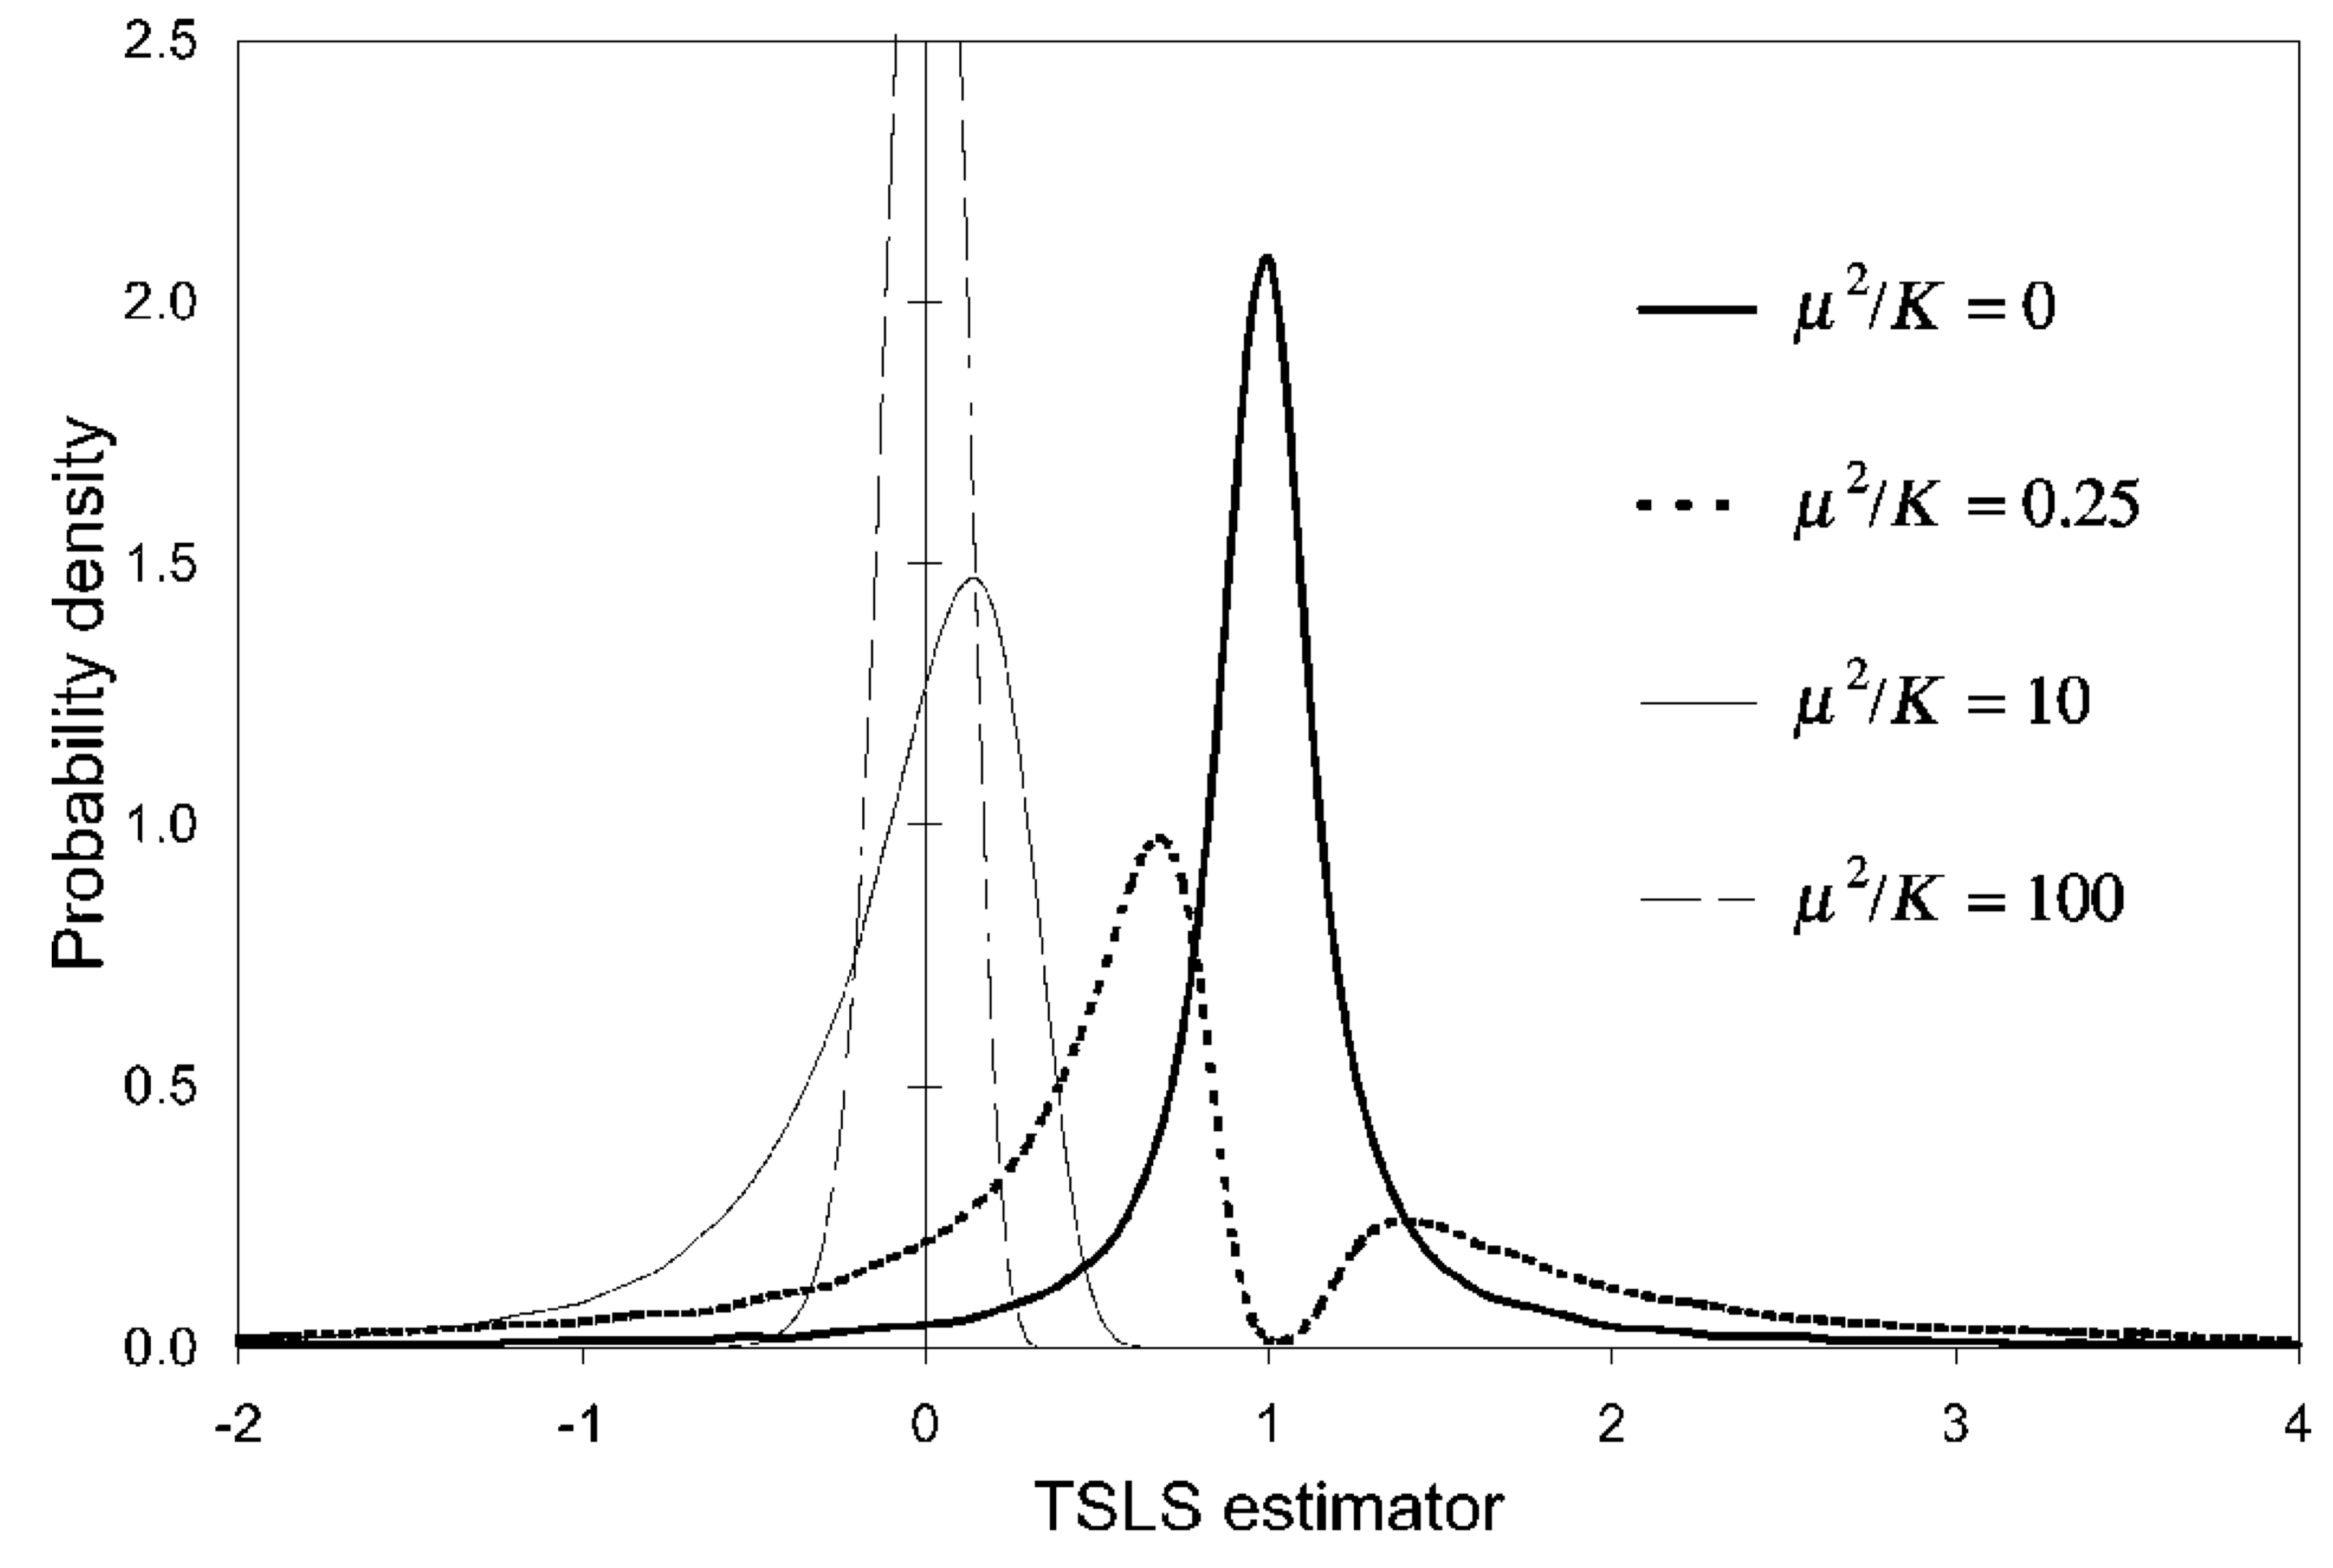
\includegraphics[width=0.49\textwidth]{figures/2sls-beta.png}
		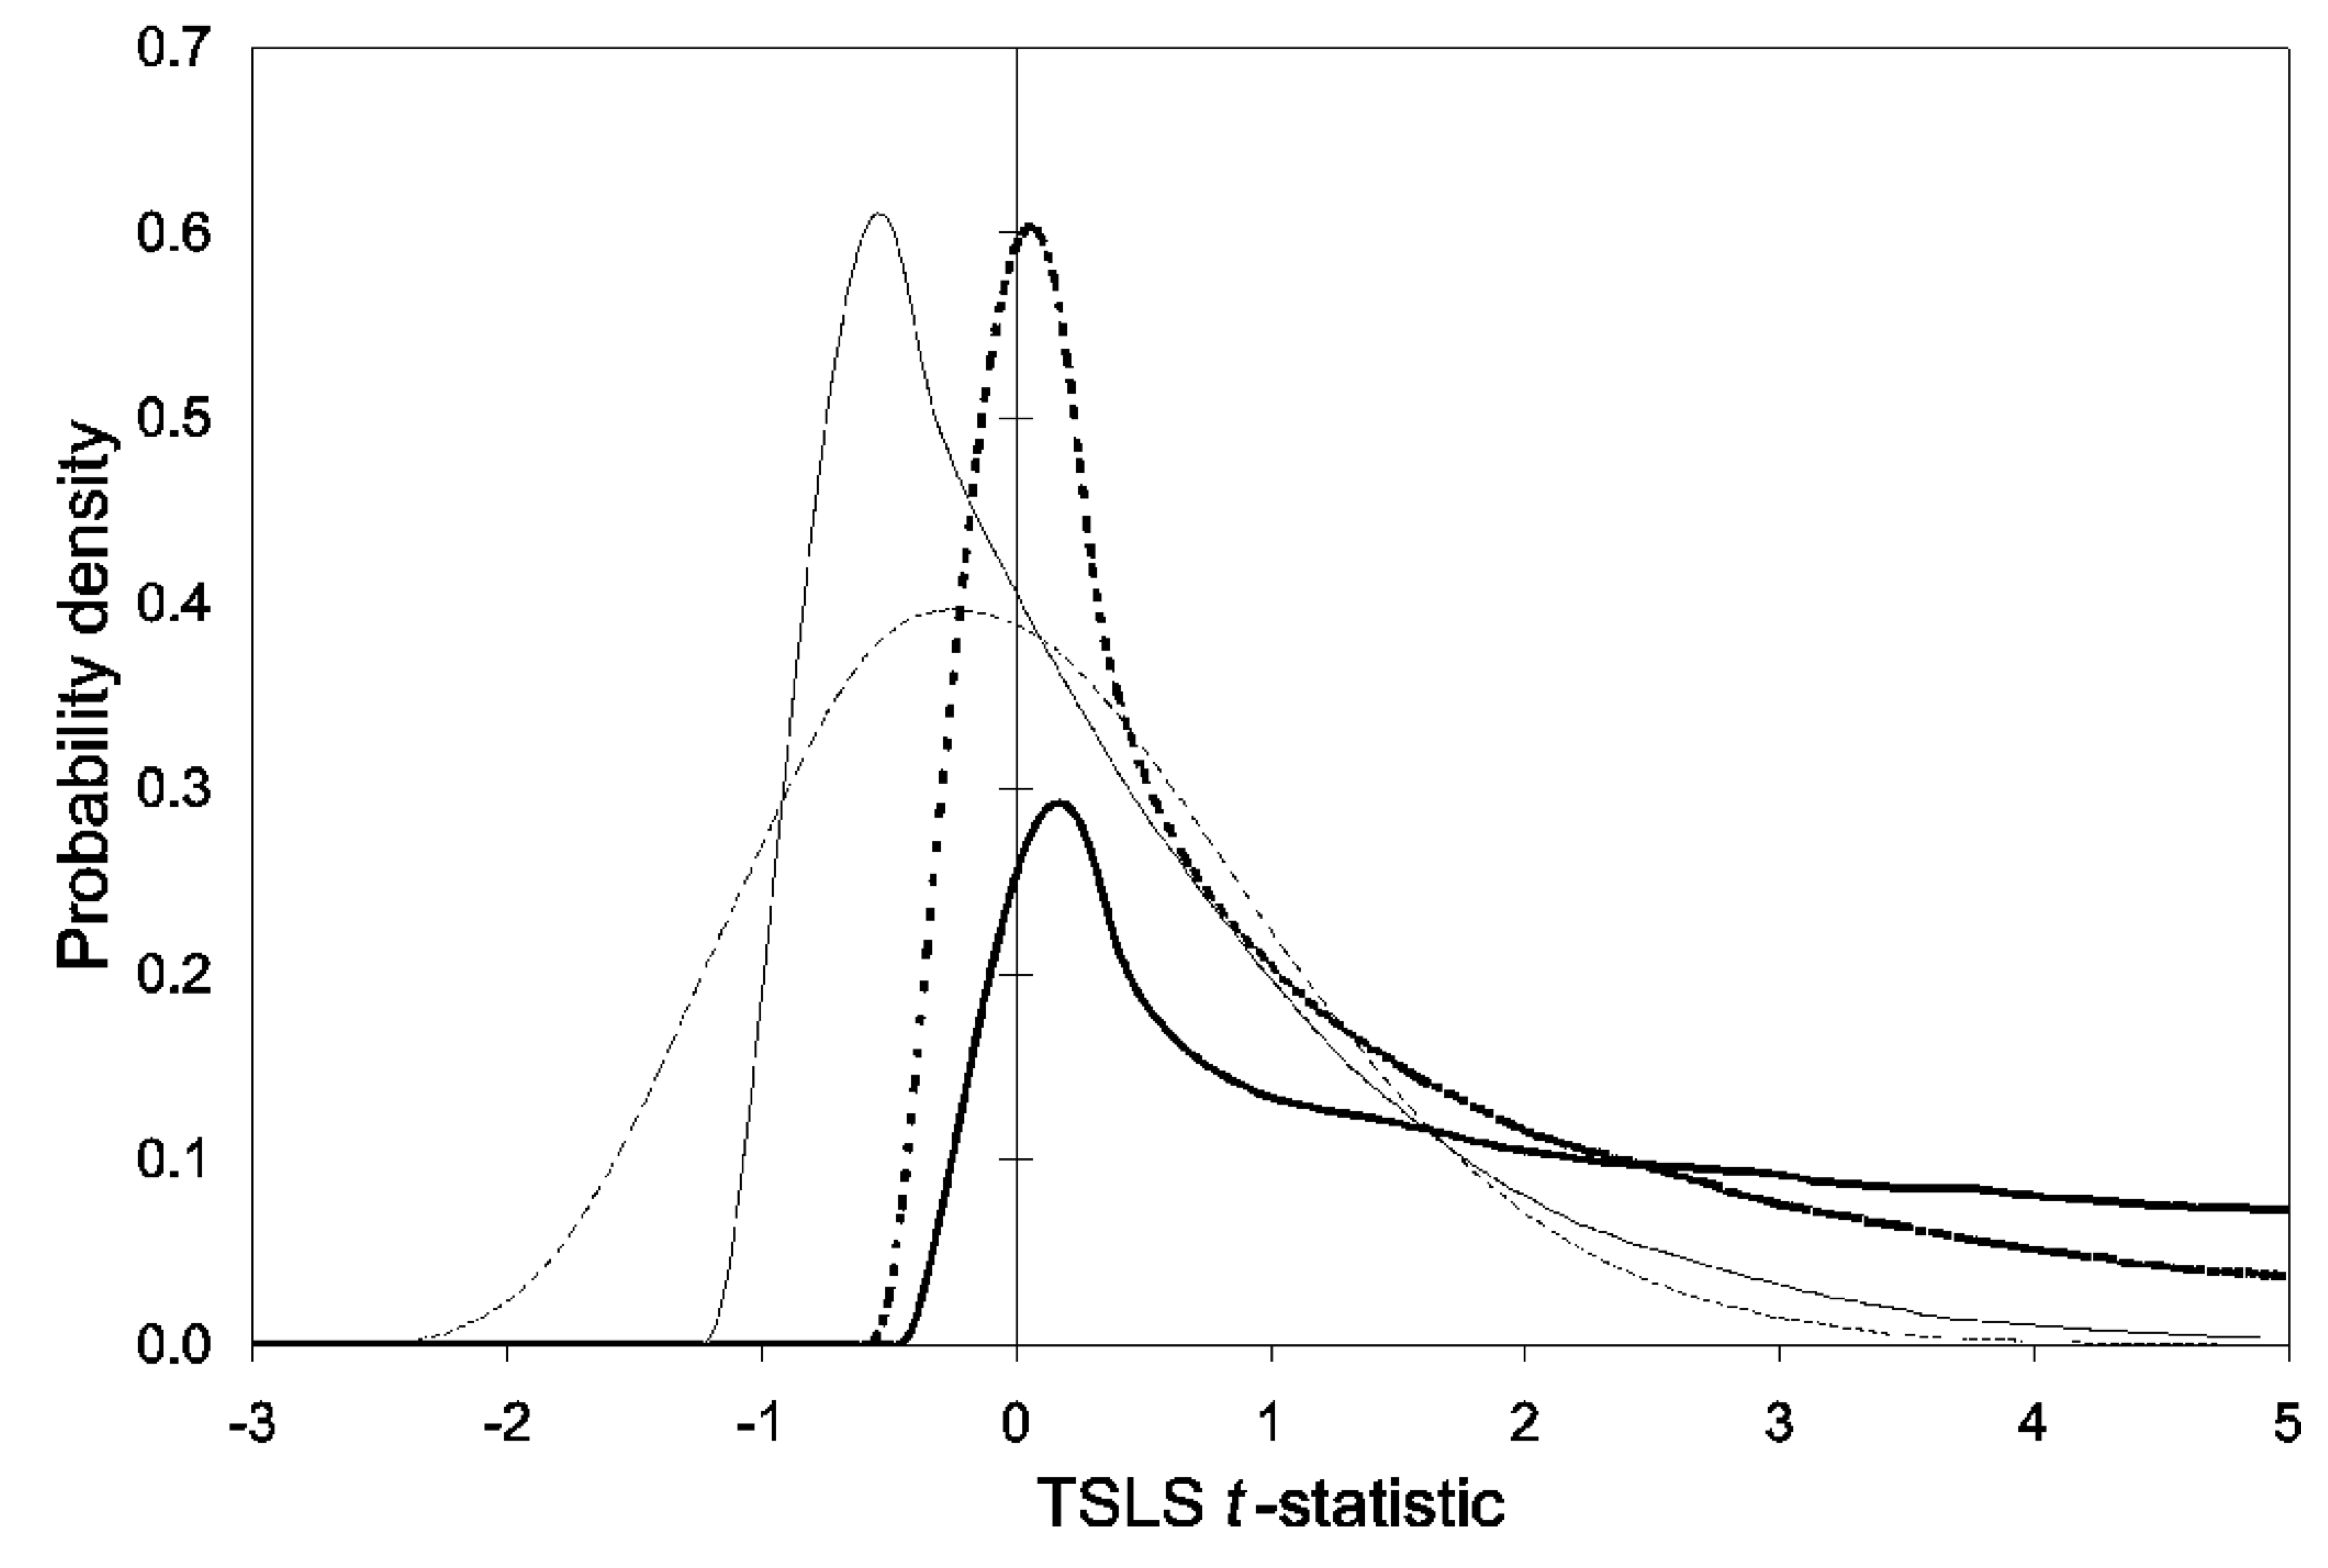
\includegraphics[width=0.49\textwidth]{figures/2sls-t-stat.png}
		\caption{Finite Sample Distributions.\vspace{3pt}\\%
		\footnotesize\emph{Source}: \textcite{stock-wright-yogo-2002}.
		More detailed versions of these densities can be found in
		\textcite{nelson-startz-1990-ecta,nelson-startz-1990-job}.}
		\label{fig:finite-sample-disttributions}
	\end{figure}
	Combining \autoref{rmk:concentration-is-effective-sample-size} and \autoref{rmk:concentration-and-f-statistic},
	one can see that a small first-stage $F$-statistic \emph{cannot} be fixed with more samples.
	However, in classic \gls*{iv} analysis, one assumes that $\PI$ is constant.
	Then, $\mu^2$ tends to infinity as $T\to\infty$, regardless of how small $\PI$ actually is.
	This is why classical \gls*{iv} asymptotic fails when instruments are weak,
	i.e., the textbook asymptotic result provides a poor approximation of the finite sample distribution.
	This problem is really brought to attention of econometricians by numerical simulations
	by \textcite{nelson-startz-1990-ecta,nelson-startz-1990-job},
	in which they demonstrated that when the concentration parameter is small,
	then the finite sample distribution \gls*{2sls} estimator and $t$-statistic are highly irregular,
	as on can see in \autoref{fig:finite-sample-disttributions}.
\end{remark}

\section{Weak \gls*{iv} Asymptotics}

Classic asymptotic results cannot capture the finite sample distribution
of the \gls*{2sls} estimator and the test statistic.
\textcite{staiger-stock-1997} provided an analysis,
now known as ``weak \gls*{iv} asymptotics,''
that successfully approximates the finite sample features using asymptotic methods.%
\footnote{
	Other asymptotic analysis of weak instruments have been developed.
	For example, ``many-instrument asymptotics'' is an asymptotic analysis
	that let the number of instruments $K$ goes to infinity.
	However,
	these kinds of asymptotics does not capture the non-normality shown in \autoref{fig:finite-sample-disttributions}.
	A more detailed survey can be found in \textcite{stock-wright-yogo-2002}.
}

The key to their asymptotic analysis is to model $\PI$ to be local to zero
by introducing a ``drift'' in the parameter $\PI$ towards $0$ as $T\to\infty$,
as described in the following assumption presented in \textcite{staiger-stock-1997}:%
\footnote{
	This technique belongs to the family of local asymptotics.
	Specifically, this kind of ``drifting'' in parameter is sometimes known as \emph{Pitman drift},
	a technique often used in power analysis of tests.
	\parencite{stock-wright-yogo-2002}
}

\begin{assumption*}[$L_{\PI}$]\label{ass:local-PI}
	$\PI = \PI_T=\CC/\sqrt{T}$, where $\CC$ is a fixed $K\times N$ matrix.
\end{assumption*}

\noindent
In the following derivations,
we still consider \gls*{iid} errors but relax the normality assumption,
since we are in the land of asymptotics.
Also, we still assume that $N=1$ for simplicity in our note.
In \textcite{staiger-stock-1997}, they consider a general $N$.

\begin{remark}
	In contrast to classic asymptotic analysis where $F$-statistic or $\mu^2$
	tends to infinity as sample size $T$ tends to infinity,
	$\mu^2$ is held constant in weak \gls*{iv} asymptotics:
	\begin{align*}
		\mu^2
		= \frac{ \PI_T\T\ZZ\T\ZZ\PI_T }{ \sigma_{\vv}^2 }
		= \frac1{\sigma_{\vv}^2} \CC\T \left(\frac{\ZZ\T\ZZ}{T}\right) \CC
		\pto \frac1{\sigma_{\vv}^2} \CC\T \QQ_{\ZZ\ZZ} \CC
	\end{align*}
	where it is (standard to) assumed that $\ZZ\T\ZZ/T$ converges in probability to a limit $\QQ_{\ZZ\ZZ}$.
\end{remark}

Under weak \gls*{iv} asymptotics, we have the limiting distribution%
\footnote{
	A detailed derivation can be found in \textcite{staiger-stock-1997}.
}
\begin{gather}\label{eq:weak-iv-asymptotic-disttribution}
	\hat\bbeta_{\text{\gls*{2sls}}} - \bbeta_0
	\dto
	\left( \frac{ \sigma_\uu }{ \sigma_\vv } \right)
	\frac{ ( \lambda + \zeta_\vv )\T \zeta_\uu }{( \lambda + \zeta_\vv )\T( \lambda + \zeta_\vv )}
	\shortintertext{where}
	\begin{bmatrix}
		\zeta_\uu \\
		\zeta_\vv
	\end{bmatrix}
	\sim
	\mathcal{N}(0,\bar\SIGMA\otimes\II_K), \quad
	\bar\SIGMA =
	\begin{bmatrix}
		1 & \rho \\
		\rho & 1
	\end{bmatrix}, \quad
	\lambda = \frac1{\sigma_\vv} \QQ_{\ZZ\ZZ}^{1/2}\CC. \nonumber
\end{gather}
Compare \eqref{eq:weak-iv-asymptotic-disttribution} to \eqref{eq:2sls-rothenberg},
one can clearly see the similarities.
Clearly, $\lambda\T\lambda$ is simply the asymptotic version of $\mu^2$.
Hence, under weak \gls*{iv} asymptotics,
one captures the finite sample features derived by \textcite{rothenberg-1984}.
% Also note that in \textcite{rothenberg-1984},
% no assumption was made about weak \gls*{iv}, whereas \textcite{staiger-stock-1997} does.
\textcite{staiger-stock-1997} also provided weak \gls*{iv} asymptotics
for the Wald statistic with $k$-class estimators.
However, since the asymptotic distributions all depend on $\lambda$
and $\lambda$ cannot be consistently estimated under this particular asymptotic setting,
the distributional results is of little use in constructing tests.

\begin{remark}[Relative Bias] % OLS bias
	Under weak \gls*{iv} asymptotics,
	then the mean of the asymptotic distribution of the \gls*{2sls} estimator is the same as the probability limit of the \gls*{ols} estimator.
	The probability limit of the \gls*{ols} estimator can be expressed as
	\begin{align*}
		\hat\bbeta_{\text{\gls*{ols}}} = (\XX\T\XX)\inv\XX\T\yy \pto \bbeta_0 + \frac{\sigma_{\vv\uu}}{\sigma_{\vv}^2}.
	\end{align*}
	Note that this result is identical to standard asymptotics with $\PI=0$.
	% If the instruments are weak but not completely irrelevant,
	% then the \gls*{2sls} estimator is biased towards the probability limit of the \gls*{ols} estimator.
	We can defined the ``relative bias'' of the \gls*{2sls} estimator as follows and calculate its expectation
	\begin{align*}
		\plim_{T\to\infty}\frac{\hat\bbeta_{\text{\gls*{2sls}}}-\bbeta_0}{\hat\bbeta_{\text{\gls*{ols}}}-\bbeta_0}
		\implies \E \left[ \plim_{T\to\infty}\frac{\hat\bbeta_{\text{\gls*{2sls}}}-\bbeta_0}{\hat\bbeta_{\text{\gls*{ols}}}-\bbeta_0} \right]
		= \E \left[ \frac{(\lambda + \zeta_{\vv})\T\zeta_{\vv}}{(\lambda + \zeta_{\vv})\T(\lambda + \zeta_{\vv})} \right].
	\end{align*}
	Due to some properties of distributional form (see footnote 4 in \textcite{staiger-stock-1997}),
	the expected relative bias only depends on $\lambda\T\lambda/K$ and $K$.
\end{remark}

% TODO: what is k-class estimator?

\begin{remark}
	Essentially,
	\textcite{staiger-stock-1997} provided an asymptotic tool,
	in contrast to previous attempts with finite samples, e.g., \textcite{rothenberg-1984},
	that makes it easier to analyze weak \gls*{iv}.
	This asymptotic in itself is not very useful in practice,
	that is, it does not provide any estimators or test.
\end{remark}

\begin{remark}
	One critical conclusion to draw from weak \gls*{iv} asymptotics is that
	$\hat\bbeta_{\text{\gls*{2sls}}}$ is inconsistent, since
	it does not converge in probability to anything.
	We have two ways to proceed:
	\begin{enumerate}
		\item
			Screen for first-stage $F$-statistic or some similar tests.
			If we are convinced that the instruments are ``strong,''
			then we can continuous with the classic \gls*{2sls} procedure
			and test $\nullhypothesis:\bbeta=0$ via the usual $t$-test.
			We need to decide when instruments are considered weak.
			\parencite{stock-yogo-2005}
		\item
			Use a fully-robust test that works regardless of whether the instruments are weak.
			We need to devise a test that is robust to the scenario that $\PI$ might be arbitrarily close to $0$.
	\end{enumerate}
	In the YouTube video \textcite{stock-2008} provided an anecdote
	that some friend of his never look at first-stage statistic and always uses fully robust inferences.
	This seems to be the trend nowadays.
\end{remark}

\section{Fully Robust Inference}

\begin{remark}
	Is there a fully robust ``estimator''?
	That is, is there some estimator $\hat\bbeta$ that is consistent regardless of instrument strength?
	Clearly not, since if $\PI=0$, $\bbeta$ is not identified.
	Hence, there is no normal $t$-test that can be performed.
	However, there are fully robust ``test'' that tests the hypothesis $\nullhypothesis:\bbeta=\bbeta_0$.
	(from \textcite{shi-2012})
\end{remark}

\noindent
There are three approaches in the literature to do fully robust inference \parencite{stock-2008}:

\begin{enumerate}[label = {A\arabic*.}]
	\item\label{item:attempt-1}
		Use a statistic that depends on $\mu^2$, but consider the worst case.
	\item\label{item:attempt-2}
		Use a statistic that does not depend on $\mu^2$.
	\item\label{item:attempt-3}
		Use a statistic that depends on $\mu^2$,
		but condition it on a computable sufficient statistic so that the conditional distribution does not depend on $\mu^2$.
\end{enumerate}

Essentially, the first approach does not work,
as the tests devised using this approach does not have any power, i.e., they are too conservative.%
\footnote{
	One such procedure, Bonferroni Confidence Region, is discussed in \textcite{staiger-stock-1997}.
	However, as mentioned in \textcite{stock-2008}, no one really pursuits this route further as it is not that useful.
}
There are two known procedures that belongs to the second approach: \glsentrylong{ar} and \glsentrylong{klm}.
The third approach is proposed by \textcite{moreira-2002},
which is the most powerful in terms of statistical power.
We will focus on \ref{item:attempt-2} and \ref{item:attempt-3} in this note.

The first fully robust inference in structural estimation is credited to \textcite{anderson-rubin-1949},
who created the \gls*{ar}.

\begin{definition}[\glsentrylong{ar}]\label{dfn:ar-1}
	\textcite{anderson-rubin-1949} proposed the \glsentrylong{ar} for testing $\bbeta=\bbeta_0$.
	\gls*{ar} is defined by
	\begin{align*}
		\text{\gls*{ar}}(\bbeta_0)
		\coloneqq
		\frac
		{ (\yy - \XX\bbeta_0)\T\PP_{\ZZ}(\yy - \XX\bbeta_0) / K }
		{ (\yy - \XX\bbeta_0)\T (\II-\PP_{\ZZ}) (\yy - \XX\bbeta_0) / (T - K) }
	\end{align*}
\end{definition}

\begin{remark}
	The original idea of \textcite{anderson-rubin-1949} is simple:
	Suppose we have the hypothesis $\nullhypothesis:\bbeta=\bbeta_0$,
	then the residual $\yy-\XX\bbeta_0$ should be uncorrelated with the instrument $\ZZ$.
	(see \textcite{stock-2008} at around \texttt{1:15:50})
\end{remark}

\begin{remark}
	$\text{\gls*{ar}}(\bbeta_0)$ has an exact $F_{K,T-K}$ distribution under $\nullhypothesis$ (of course, only under finite sample normality).
	Also, under weak \gls*{iv} asymptotics,
	$\text{\gls*{ar}}(\bbeta_0)$ converges in distribution to $\chi_{K}^2/K$ under $\nullhypothesis$,
	regardless of the size of $\mu^2$.
	\parencite{stock-wright-yogo-2002}
\end{remark}

\begin{remark}[Robust Confidence Region]
	Using \gls*{ar},
	we can construct a robust confidence region of $\bbeta$
	by collecting all $\bbeta_0$ such that $\text{\gls*{ar}}(\bbeta_0)$ fails to reject.
	\parencite{staiger-stock-1997}
\end{remark}

\begin{remark}
	\gls*{ar} is a uniformly most powerful test when $K=1$ \parencite{moreira-2009}.
	However, the power of \gls*{ar} is low when $K>1$.
	% TODO: explain?
\end{remark}

\begin{remark}
	\gls*{ar} can reject either due to $\bbeta\neq\bbeta_0$ or due to non-exogenous variables.
\end{remark}

%%%%%%%%%%%%%%%%%%%%%%%%%%%%%%%%%%%%%%%%%%%%%%%%%%%%%%%%%%%%%%%%%%%%%%%%%%%%%%%

Before moving on to the statistic proposed by \textcite{kleibergen-2002},
we should take a look at \textcite{moreira-2009} to better understand
how these ``fully-robust'' tests are constructed.%
\footnote{
	A manuscript of \textcite{moreira-2009} appeared as early as 2001.
}

\textcite{moreira-2009} considered the following setting:
The reduced form of the \gls*{iv} model is $\yy = \XX\bbeta + \uu = \ZZ\PI\bbeta + \tilde\vv$
where $\tilde\vv = \uu + \vv\bbeta$.
Let $(\tilde\vv_t,\vv_t)$ be a bivariate normal distribution with \emph{known}, for now, covariance matrix $\OMEGA$.
We are interested in the hypothesis $\nullhypothesis:\bbeta=\bbeta_0$.
This probability model belongs to the (curved) exponential family,
hence, $\ZZ\T[\yy,\XX]$, or $\ZZ\T[\yy,\XX]D$ for any invertible $D$,
is a sufficient statistic for the pair $(\bbeta,\PI)$.
A convenient choice of $D$ is to let $D=[b_0,a_0]$
where $a_0=(\bbeta_0,1)\T$ $b_0=(1,-\bbeta_0)\T$.
With some appropriate scaling, we have that
\begin{align}
	\mathcal{S} = \frac{ (\ZZ\T\ZZ)^{-1/2}\ZZ\T[\yy,\XX]b_0 }{ \sqrt{b_0\T\OMEGA b_0} } \quad\text{and}\quad
	\mathcal{T} = \frac{ (\ZZ\T\ZZ)^{-1/2}\ZZ\T[\yy,\XX]\OMEGA\inv a_0 }{ \sqrt{a_0\T\OMEGA a_0} }
\end{align}
are sufficient for the pair $(\bbeta,\PI)$.%
\footnote{
	This particular set of $\mathcal{S}$ and $\mathcal{T}$ appeared in \textcite{stock-wright-yogo-2002}.
	Similar definitions can also be found, of course, in \textcite{moreira-2009}.
}

\begin{remark}
	Since $\mathcal{S}$ and $\mathcal{T}$ are sufficient for $(\bbeta,\PI)$,
	we can consider only functions of $\mathcal{S}$ and $\mathcal{T}$ when constructing tests.
	Notice that in $\mathcal{S}$, we have the term $[\yy,\XX]b_0$, which evaluates to $\uu$ under $\nullhypothesis$.
	Therefore, $\mathcal{S}$ does not depend on $\PI$ under the null hypothesis $\nullhypothesis$.
	This is the key why we can construct fully robust tests.
	\parencite{stock-wright-yogo-2002}
\end{remark}

\begin{remark}
	Since $\mathcal{S}$ does not depend on $\PI$ under $\nullhypothesis$,
	$\mathcal{T}$ is sufficient for $\PI$ under $\nullhypothesis$.
	It follows that a test of $\bbeta=\bbeta_0$ based on some function $g(\mathcal{S},\mathcal{T})$ is \emph{similar}
	if its critical value is computed from the conditional distribution of $g(\mathcal{S},\mathcal{T})$ given $\mathcal{T}$.
	In this context,
	\emph{similar} simply means that the distribution of the test statistic does not depend on the nuisance parameter $\PI$.
	\footnote{
		See \textcite{lehmann-2022} \emph{Chapter 4 Unbiasedness: Theory and First Applications}
		for details about statically similar tests.
	}
	\parencite{moreira-2009,stock-wright-yogo-2002}
\end{remark}

\begin{remark}
	Furthermore, one can show that $\mathcal{S}$ and $\mathcal{T}$ are independent normal distributions.
	Hence the conditional distribution of $g(\mathcal{S},\mathcal{T})$ is obtained
	simply by replacing $\mathcal{T}$ with the conditioned value.
	And since the conditional distribution of $g(\mathcal{S},\mathcal{T})$ does not depend on $\PI$
	(since $\mathcal{S}$ does not depend on $\PI$),
	it is a pivotal and its distribution is known (or at least can be computed with simulation).
	\parencite{moreira-2009,shi-2012}
\end{remark}

\begin{remark}
	In practice, the value of $\OMEGA$ is not known.
	However, we can easily estimate it using $\hat\OMEGA=[\yy,\XX]\T(\II-\PP_\ZZ)[\yy,\XX]/(T-K)$.
	Henceforth, we will denote the ``$\hat\OMEGA$ plugged-in'' versions of $\mathcal{S}$ and $\mathcal{T}$
	as $\hat{\mathcal{S}}$ and $\hat{\mathcal{T}}$ respectively.
	\parencite{stock-wright-yogo-2002}
\end{remark}

Now we can rewrite \autoref{dfn:ar-1} as follows

\begin{definition}[\glsentrylong{ar}]\label{dfn:ar-2}
	The \glsentrylong{ar} is defined as
	\begin{align*}
		\text{\gls*{ar}}(\bbeta_0)
		= \frac1K \hat{\mathcal{S}}\T \hat{\mathcal{S}}
	\end{align*}
\end{definition}

\begin{remark}
	It is quite clear why \gls*{ar} is robust:
	$\mathcal{S}$ does not depend on the value of $\PI$ under $\nullhypothesis$.
	However, we now see a potential room for improvement:
	since we need to have both $\mathcal{S}$ and $\mathcal{T}$ to fully extract the information of $\bbeta$ and $\PI$,
	we must somehow incorporate the set $\mathcal{S}$ and $\mathcal{T}$ in the test statistic.
\end{remark}

\begin{definition}[\glsentrylong{klm}]
	\textcite{kleibergen-2002} proposed the \gls*{klm} as
	\begin{align*}
		\text{\gls*{klm}}(\bbeta_0) = \frac{ ( \hat{\mathcal{S}}\T\hat{\mathcal{T}} )^2 }{ \hat{\mathcal{T}}\T\hat{\mathcal{T}} }
	\end{align*}
\end{definition}

\begin{remark}
	When $K=1$, then $\text{\gls*{klm}}(\bbeta_0)$ and $\text{\gls*{ar}}(\bbeta_0)$ are equivalent.
\end{remark}

\begin{remark}
	$\text{\gls*{klm}}(\bbeta_0)$ has
	standard/weak \gls*{iv} asymptotic of $\chi_{1}^2$ limiting distribution under $\nullhypothesis$.
	It is remarkable that the asymptotic distribution of \gls*{klm} is free of $\PI$,
	even though $\mathcal{T}$ is present.
	One way to see that the asymptotic distribution of \gls*{klm} does not depend on $\mathcal{T}$ is to check that
	for all values of $\mathcal{T}$, \gls*{klm} has the same asymptotic distribution $\chi^2_1$.
	% TODO: how? Shi
\end{remark}

\begin{remark}
	Compared to the asymptotic distribution of \gls*{ar},
	which has $\chi_{K}^2/K$ limiting distribution,
	$\text{\gls*{klm}}(\bbeta_0)$ has higher power when $K$ is large since it has constant degree of freedom.
	% TODO: explain?
\end{remark}

\begin{remark}
	However, one major downside of \gls*{klm} is that it has weird power qualities.
	That is, the test statistic is non-monotone in $|\bbeta-\bbeta_0|$ in some cases.
	Also, the power of it is dominated by the statistic proposed by \textcite{moreira-2002}.
	Thus in \textcite{stock-2008}, Stock said that he does not like \gls*{klm}.
\end{remark}

\begin{definition}[\citeauthor{moreira-2002} Statistic]
	\textcite{moreira-2002} proposed the following \gls*{clr}
	\begin{align*}
		\text{\gls*{clr}}(\bbeta_0) = \frac12
		\left(
		\hat{\mathcal{S}}\T\hat{\mathcal{S}}
		- \hat{\mathcal{T}}\T\hat{\mathcal{T}}
		+
		\sqrt{
		( \hat{\mathcal{S}}\T\hat{\mathcal{S}} + \hat{\mathcal{T}}\T\hat{\mathcal{T}} )^2
		- 4 \cdot
		\left(
		(\hat{\mathcal{S}}\T\hat{\mathcal{S}}) (\hat{\mathcal{T}}\T\hat{\mathcal{T}})
		- (\hat{\mathcal{S}}\T\hat{\mathcal{T}})^2
		\right)
		}
		\right)
	\end{align*}
	conditional on $\hat{\mathcal{T}}$.
\end{definition}

\begin{remark}
	The standard/weak \gls*{iv} asymptotic distribution of $\text{\gls*{clr}}(\bbeta_0)$,
	condition of $\hat{\mathcal{T}}$, is non-standard,
	and depends on $\bbeta_0$ and $\hat{\mathcal{T}}$.
	\textcite{moreira-2002} suggests to compute the asymptotic distribution with Monte Carlo simulation.
\end{remark}

% \begin{remark}
% 	In power analysis in \textcite{stock-wright-yogo-2002},
% 	one can see that $\text{\gls*{clr}}(\bbeta_0)$ almost always has more power compared to $\text{\gls*{klm}}(\bbeta_0)$,
% 	and the power of $\text{\gls*{clr}}(\bbeta_0)$ hugs theoretical maximum power more closely.
% 	(See section 5.4 in \textcite{stock-wright-yogo-2002})
% \end{remark}

\begin{remark}
	\parencite{stock-2008}
	The problem of testing $\nullhypothesis:\bbeta=\bbeta_0$ when $N=1$ is essentially solved by \gls*{clr} in practice.
	In simulations studies, \gls*{clr} is practically the uniformly most powerful test,
	since it closely hugs the theoretical power envelop.
	It is more powerful than \gls*{ar} and \gls*{klm}.
\end{remark}

\section{Further Topics}

\begin{enumerate}
	% \item
	% 	Complete and Similar tests.
	\item
		\gls*{liml} and $k$-class estimators: A more robust form of \emph{estimation} compared to \gls*{2sls}.
	\item
		Implications in \gls*{gmm}.
\end{enumerate}

\printglossaries
\printbibliography

\end{document}
